\documentclass{article}
\PassOptionsToPackage{numbers, compress}{natbib}

% if you need to pass options to natbib, use, e.g.:
%     \PassOptionsToPackage{numbers, compress}{natbib}
% before loading neurips_2022


% ready for submission
\usepackage{neurips_2022}
\usepackage{algorithm2e}
\usepackage{amsmath}
\usepackage{geometry}
\geometry{verbose,letterpaper}
\usepackage{movie15}
\usepackage{hyperref}
\usepackage{graphicx}

% to compile a preprint version, e.g., for submission to arXiv, add add the
% [preprint] option:
%     \usepackage[preprint]{neurips_2022}


% to compile a camera-ready version, add the [final] option, e.g.:
%     \usepackage[final]{neurips_2022}


% to avoid loading the natbib package, add option nonatbib:
%    \usepackage[nonatbib]{neurips_2022}]


\usepackage[utf8]{inputenc} % allow utf-8 input
\usepackage[T1]{fontenc}    % use 8-bit T1 fonts
\usepackage{hyperref}       % hyperlinks
\usepackage{url}            % simple URL typesetting
\usepackage{booktabs}       % professional-quality tables
\usepackage{amsfonts}       % blackboard math symbols
\usepackage{nicefrac}       % compact symbols for 1/2, etc.
\usepackage{microtype}      % microtypography
\usepackage{xcolor}         % colors


\title{Adapting Diffusion-LM to Discrete Music Domain}


% The \author macro works with any number of authors. There are two commands
% used to separate the names and addresses of multiple authors: \And and \AND.
%
% Using \And between authors leaves it to LaTeX to determine where to break the
% lines. Using \AND forces a line break at that point. So, if LaTeX puts 3 of 4
% authors names on the first line, and the last on the second line, try using
% \AND instead of \And before the third author name.


\author{%
  Janavi Kasera\\
  \texttt{jkasera@bu.edu} \\
  % examples of more authors
  \AND 
  Ruiqi Liu\\
  \texttt{ruiqiliu@bu.edu} \\
  \AND
  Chuhan Li \\
  \texttt{lich@bu.edu} \\
}


\begin{document}


\maketitle


\begin{abstract}

In recent years, music or audio generation and synthesis have become a sought after challenge in the world of data generation. Current methods of music generation are divided into two channels - (a) capitalizing auto-regressive models to generate music in the continuous domain, and (b) the use of non auto-regressive models to produce music represented in discrete space. Lately, using text-based language models to produce discrete domain music has gained a lot of prominence. Music when represented discretely is a sequence of tokens (symbols) depicting different music information such as pitch, frequency, velocity, bass, and so on, for each musical note at different intervals in time. Leveraging on the sequential nature of the discrete domain music, we propose to adapt a novel state-of-the-art language model, \textit{Diffusion-LM}, to generate piano sounds. 

\end{abstract}


\section{Introduction}

In recent years, language models have demonstrated their exceptional generative abilities (such as, open-ended dialogue, machine translation, and so on). Likewise, these models have also proved their proficiency in generating other signals different than texts, such as natural images and audio signals. This is the key intuition behind our project. Given that language models use the sequential nature of its training data to make predictions/generations, in this project we used the symbolic representation of music as training data, and re-trained the entire \textit{Diffusion-LM} model to generate new piano music. 

Symbolic music is a token representation of audio sequences and belongs to the discrete domain. Usually, such representation requires tokens for when each note (say C, D, E, F, G) begins, what are the characteristic properties (such as velocity, frequency, pitch, and so on) of that note, and when the note ends. As such, in recent research and industrial applications, the use of MIDI files as a symbolic representation of music has proven to be an effective source of data expression. By the same token, in this project, we used over 10,000 different MIDI representations of different piano sounds to train our model. 

Though the MIDI file represents music as a sequence of tokens, the MIDI file itself cannot be directly fed into the Diffusion-LM model. There needs to be an encoding or parsing system/methodology that takes each symbol in the MIDI file and converts them into a sequence of characters that can be written in a text file. Therefore, this facilitates the generation of more readable data to can be fed into the language model. While, token embedding systems like LahkNES, MusicVAE, and MuseNet exists, for our project we took inspiration from the mmmtrack encoding system [12]. Section 4.1 of the paper discusses more on the data and encoding system used. 

The other key area of focus of our project is to also identify methods of adaptation of \textit{Diffusion-LM} model to generate audio. Particularly, we experimented with the inclusion of different transformer models within the Diffusion-LM architecture, \textit{BERT and ELECTRA-BERT}, to test the fluctuations in music quality, melody rhythm, overfitting of the model, and optimization power between the two versions of the architecture (Section 4.2 of the paper describes in detail the architecture of the model used in the project). 


\section{Related Work}

In the past, audio generation and synthesis have mainly come under the realm of autoregressive and generative models. Particularly, with the introduction of models such as WaveNet [2] and Jukebox [4], a new autoregressive classification approach to audio synthesis exists that significantly outperforms traditional concatenative and parametric approaches to audio synthesis. While Jukebox [4] uses Hierarchical Vector Quantized Variational Autoencoder (VQ-VAE architecture) to encode raw samples, WaveNet [2] is an audio generative model based on PixelCNN [13]. Some other research works have employed Generative Adversarial Models to generate audio sequences. These models, such as Spec-GAN [3] and GANSynth [6], take in their audio inputs in the form of waveforms and spectrograms and generate fixed length audio sequences. Though the aforementioned models have been successful in generating high-quality audio samples, their output belongs to the continuous domain. Owing to their Langevin-inspired sampling mechanisms, these models' application to discrete symbolic music data is very limited. 

To combat this issue, two very different research developments- AudioLM [14] and Symbolic Music Generator [15] have been made in the past year. While AudioLM [14] maps input audio (in waveform, i.e. in continuous domain) to a sequence of discrete tokens that is passed into a language model for audio generation in the representative space, Symbolic Music Generator [15] directly deals with symbolic music data (such as, MIDI files) by parameterizing the discrete domain in the continuous latent space of a pre-trained variational autoencoder. Both the models above offer a framework for high-quality audio generation with long-term consistency. On one hand, AudioLM creates a tokenized mapping from continuous to discrete space to produce audio that leverages the language model's ability to capture the syntactic and semantic properties of the text (or in the case of music, its melodies and pitches), on the other hand, Symbolic Music Generator capitalizes on the creation of a unique latent embedding that is iteratively trained on a VAE to unconditional generation and post-hoc conditional infilling. 

Thus, drawing inspiration from the above two bodies of work, we propose a novel way to use the state-of-the-art language model, \textit{Diffusion-LM} for audio generation. Drawing from [15], we propose to use MIDI files (representatives of discrete audio) as inputs to a language model. Thus, our approach combines the use of symbolic music (as in [15]) to be fed into a language model (as in [14]) to generate high-quality melodies. \textit{Diffusion-LM} optimizes in fine-grained control (such as, syntactic structures) that outperforms all the other prior works [16]. 


\section{Problem Formulation}

As mentioned above, previous work on audio generation either focuses on audio generation from continuous music data or on constructing an embedding system that can map discrete music to a continuous latent space which is used by a VAE to generate music. In our project, we propose to apply discrete music to a language generative model to produce music. In other words, our proposed methodology involves taking in the audio in discrete form and encoding it into a sequence of characters that can be fed into the language model to produce a new sequence of music characters, that can in turn be converted back to an audio form. In the following subsections, we will now examine the major components of the Diffusion-LM model. 

\subsection{Controllable Text Generation}

The text generation task is the task of sampling $\vec{w} = \{w_1, w_2, \cdots, w_n\}$ from a trained language model $p_{LM}(\vec{w})$, where $w_i \in \vec{w}$ denotes the probability of word $i$. Given the uncertainty of the generation model, it is significant and worthwhile to generate text from a given domain $c$. In this way, the controllable text generation is the task of sampling $\vec{w}$ from a domain $c$, i.e., $p(\vec{w}|c)$. Denote $c$ as the controllable variable, where $c$ could be the specific genre of music, the sentiment of music, or the style of music. With Baye's rule, we have $p(\vec{w} | c) \propto p(c | \vec{w}) \cdot p_{LM}(\vec{w})$. Given this, we are sampling the posterior from the language model prior and the genre (sentiment or style) classifier $p(c | \vec{w})$. Note $p(c | \vec{w})$ can be easily obtained by basic sequential models using labeled music training data. 

\subsection{Autoregressive Model}

The canonical approach to language modeling factors $p_{lm}$ in an autoregressive model is $p_{lm}(\mathbf{w}) = p_{lm}(\mathbf{w_1}) \prod_{i=2}^{n} p_{lm}(\mathbf{x_i |x_{<i}}) $
In this case, text generation is reduced to the task of repeatedly predicting the next token conditioned on the partial sequence generated so far. In fact, autoregressive models are merely feed-forward models, which means the context words are only in two directions, forward and backward. However, for music data, there can be multiple notes at the same time, implying the presence of the third dimension of depth which the model is unable to capture. Thus, to better handle the problem that music could have multiple notes at the same time, we are not using an autoregressive model.

\subsection{Continuous Diffusion Model}

Diffusion model is a latent variable model that models the data using Markov chain, $x_0, x_1, \cdots, x_T$. Diffusion model gradually add Gaussian noise at each step of $p(x_t | x_{t-1})$, and then reverse the model. We summarize the 1-step transition probability and $T$-step transition probability below:

$$q(x_t|x_{t-1}) = \mathcal{N}(x_t; \sqrt{1 - \beta_t}x_{t-1}, \beta_t I)$$
$$q(x_{1:T}|x_0) = \prod\limits_{t=1}^{T}q(x_t|x_{t-1})$$
$$p_{\theta}(x_{t-1}|x_t) = \mathcal{N}(x_{t-1};\mu_{\theta}(x_t, t), \Sigma_{\theta}(x_t, t)$$

\begin{figure}[!htb]
   \begin{minipage}{1\textwidth}
     \centering
     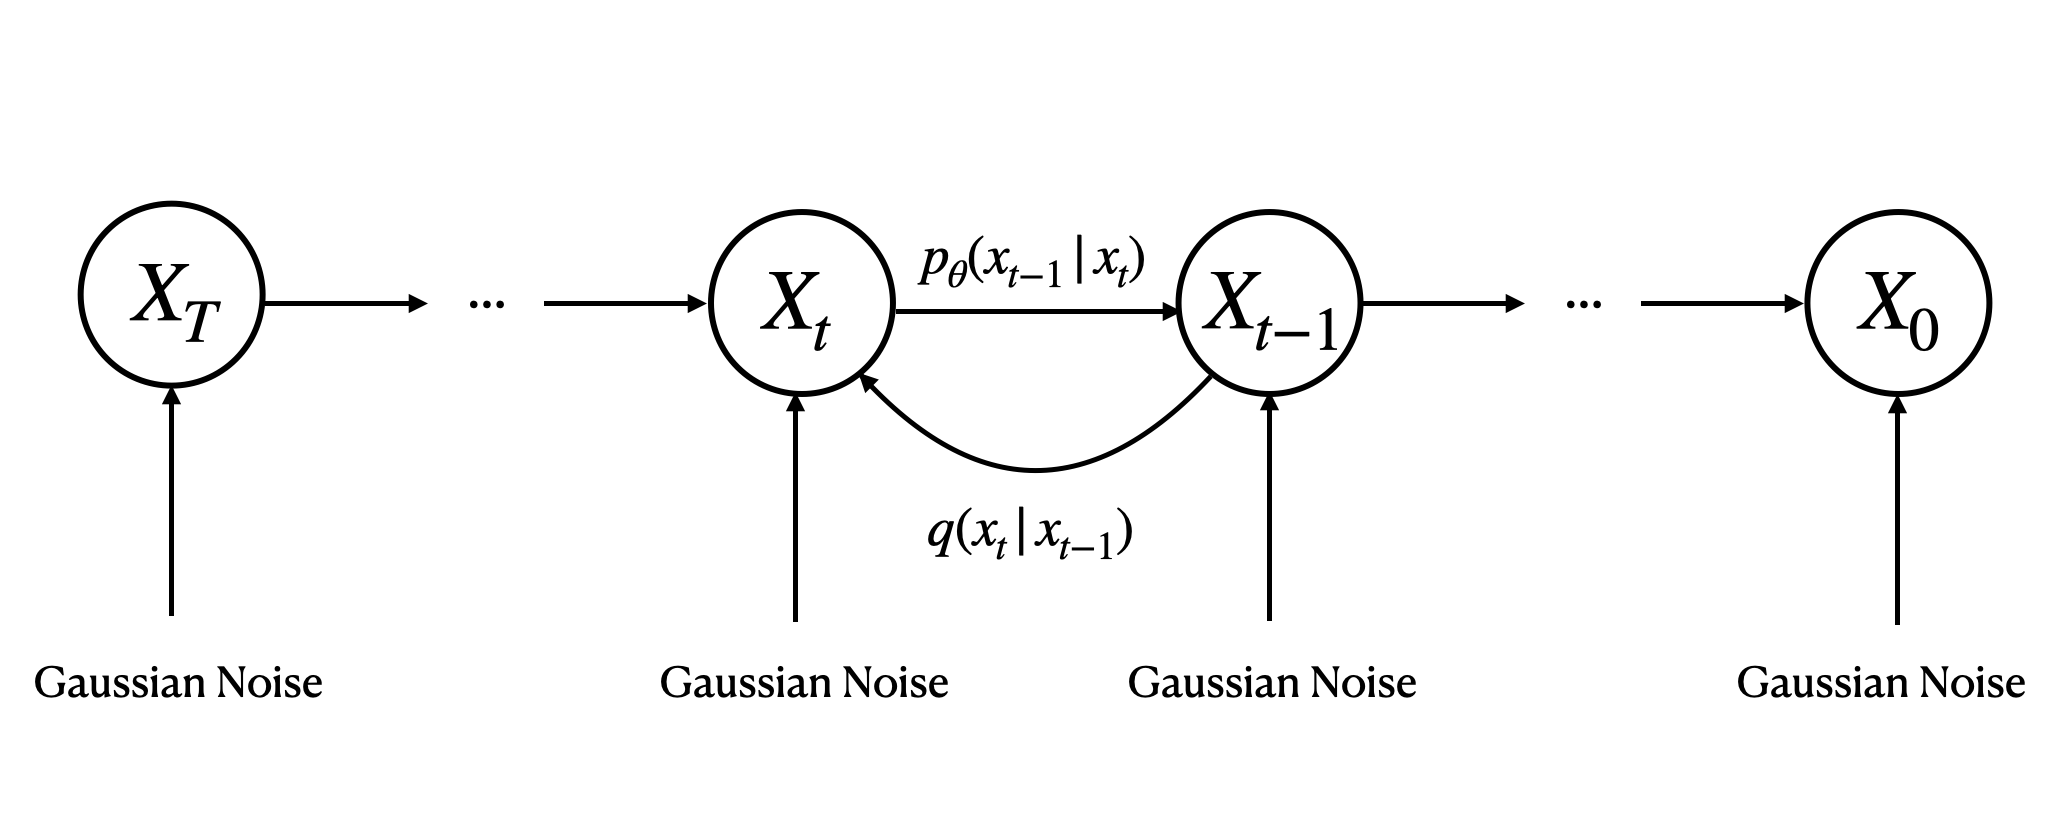
\includegraphics[width=\linewidth]{diffusion_model.png}
     \caption{Graphical representation of the diffusion model. In state $x_{t-1}$, we add Gaussian noise to transit it into state $x_t$. The amount of noise is denoted by $\beta_t$.}\label{Fig:Data1}
   \end{minipage}\hfill
\end{figure}


The diffusion model aims to minimize the variational lower bound (VLB) calculated as follows:
$$\mathcal{L}_{VLB} = 
\mathbb{E}_q[
D_{KL}(q(x_T|x_0) \| p_{\theta}(x_T)) 
+ 
\sum\limits_{t = 2}^{T}
D_{KL}(
q(x_{t-1}|x_t, x_0)
\|
p_{\theta}(x_{t-1}|x_t)) 
- 
\log p_{\theta}(x_0|x_1)
]$$

Since VLB is not stable, Ho et al [8] provide a new loss function that is much simpler than VLB. It is defined as follows: 

$$\mathcal{L}_{simple}(\theta) := \mathbb{E}_{t, x_0, \epsilon}[\|
\epsilon - \epsilon_{\theta}(\sqrt{\bar{\alpha_t}}x_0 +
\sqrt{1 - \bar{\alpha_t}}\epsilon, t)
\|^2]$$


\section{Methods}

We now discuss the different components used in our project. 

\subsection{Data Pre-processing and Token Encoding}

We used the Lakh Large MIDI dataset, which contains more than 10,000 piano MIDI files to generate piano music. Since parsing the information contained in the MIDI file to an appropriate sequential representation in the text file is an important step in our project, we utilized a token encoding system inspired by the mmmtrack encoding system [12]. 


To fully capture the information from MIDI file, we extract the information regarding pitch, velocity, and duration of each note and parse it to a text file using the encoding- $p\square\square$, $v\square\square$, and $d\square\square$, where $\square$ denotes the placeholder to represent the note's pitch, velocity, and duration, respectively. If there are multiple notes appearing simultaneously, we "compress" them and made them a series of notations. 

Since it is difficult to pre-process MIDI file directly, we pre-process the text file generated by MIDI. In the pre-processing stage, we clamp the note with extremely high or low pitch and add {\tt{[CLS]}} and {\tt{[SEP]}} to denote the beginning and the ending of the text file. For example, if the original text file has 128 words, there will be 130 words (plus {\tt{[CLS]}} and {\tt{[SEP]}}) in the processed text. 

\subsection{Diffusion-LM}

Since the original diffusion model is for continuous modeling and the text-generating task is in the discrete space, we need to find the way to map the discrete text to the continuous diffusion model. To address this, [7] proposed an end-to-end training objective for learning word ebeddings. After that, we need to map the word embeddings back to words. [7] proposed a training and decoding time methods to facilitate the mapping function. 

Compared to the random Gaussian embeddings or the pre-trained word embeddings, end-to-end training in [7] is the optimal. We add the text next to the $x_0$ state. In the forward pass, the transition function is $q(x_0|Text) = \mathcal{N}(Embedding(Text), \sigma_0 I )$. In the reverse pass, we add the trainable rounding step, parameterized by $p_{\theta}(Text|x_0) = \prod\limits_{i=1}^{n} p_{\theta}(Text_i|x_i)$, where the last term is the softmax distribution. The trainable step is described below:

$$\mathcal{L}_{vlb}^{e2e}(Text) = \sum\limits_{q_{\phi}(x_0 | Text)}
[\mathcal{L}_{vlb}(x_0) + \log q_{\phi}(x_0|Text) - \log p_{\theta}(Text|x_0)]$$
$$\mathcal{L}_{simple}^{e2e}(Text) = \sum\limits_{q_{\phi}(x_{0:T} | Text)}
[\mathcal{L}_{simple}(x_0) + \|Embedding(Text) - \mu_{\theta}(x_1, 1)\|^2
- \log p_{\theta}(Text|x_0)]$$

The second step is to get the word from word embeddings. We re-parametrized $\mathcal{L}_{simple}$ to make the model learnable in terms of $x_0$, i.e., 
$\mathcal{L}_{x_0-simple}^{e2e}(x_0) 
= \sum\limits_{t=1}^{T}\mathbb{E}_{x_t}\|f_{\theta}(x_t, t) - x_0\|^2$, where it can be used to predict $x_0$.

The overall diffusion-LM proposed by [7] contains a controllable generation. In our model, we removed the controlled generation in the diffusion-LM and replace it by the uncontrolled generation. 



\subsection{BERT vs. ELECTRA-BERT} 
To further explore the potentials of current architecture, we deployed Electra-Bert [10] as the based network in reversing process of diffusion model. In consider the size of our dataset, deploying Electra-Bert can bring 2 benefits. Firstly, Electra-Bert is a more light weight model compared to Bert, so it might be a better suit in trainning on our dataset and generate a better result. Second, it can be trained in a relatively faster way compared to Diffusion model using Bert. The following are the illustration of Diffusion-LM architecture we adapted. 

\begin{figure}[!htb]
   \begin{minipage}{1\textwidth}
     \centering
     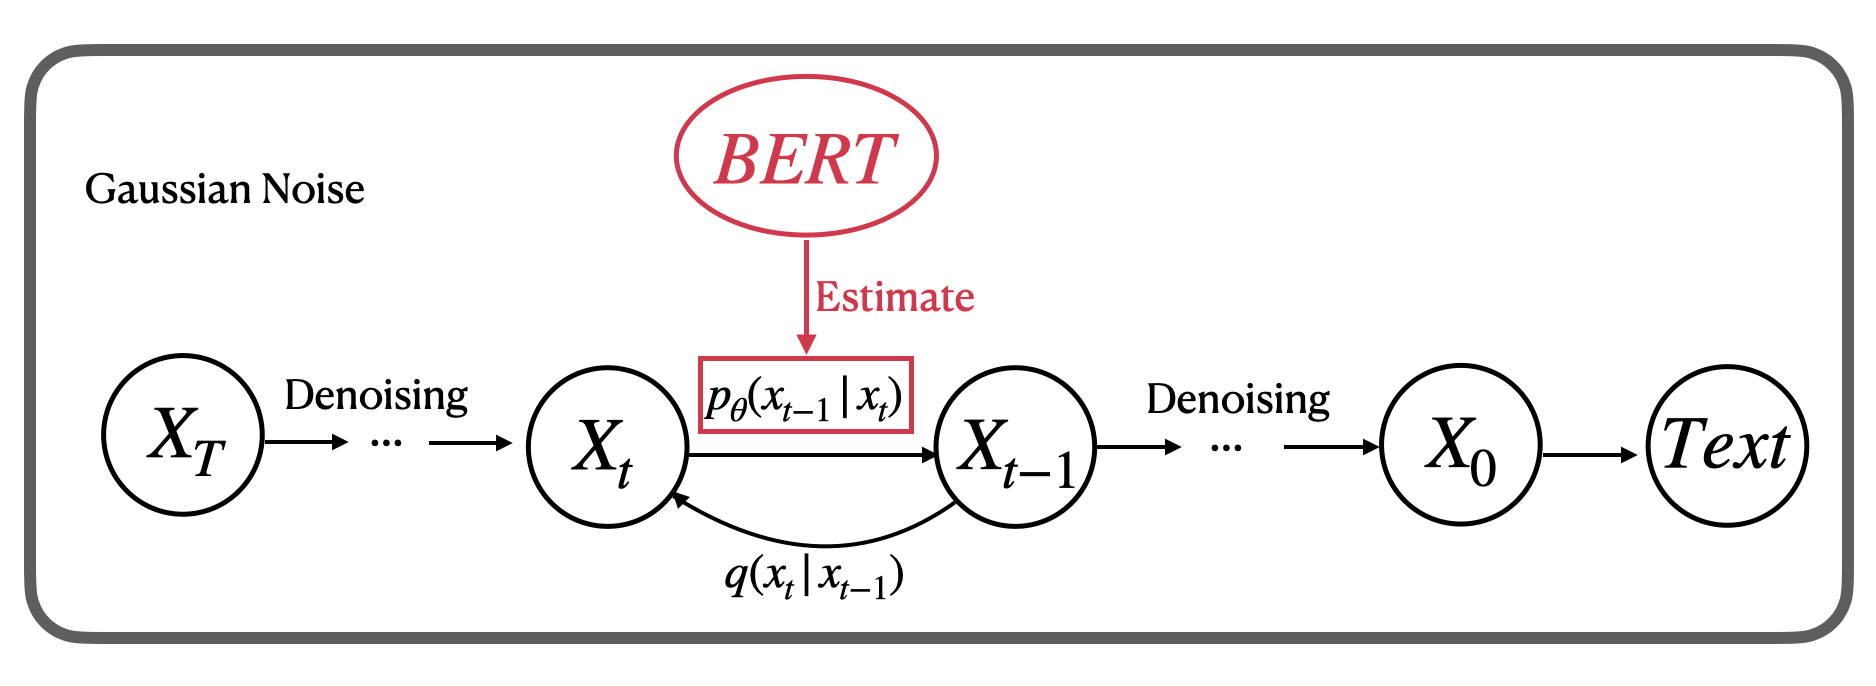
\includegraphics[width=12cm]{BERT.png}
     \caption{Graphical representation of the diffusion model with BERT.}\label{Fig:Data1}
   \end{minipage}\hfill
\end{figure}

\begin{figure}[!htb]
   \begin{minipage}{1\textwidth}
     \centering
     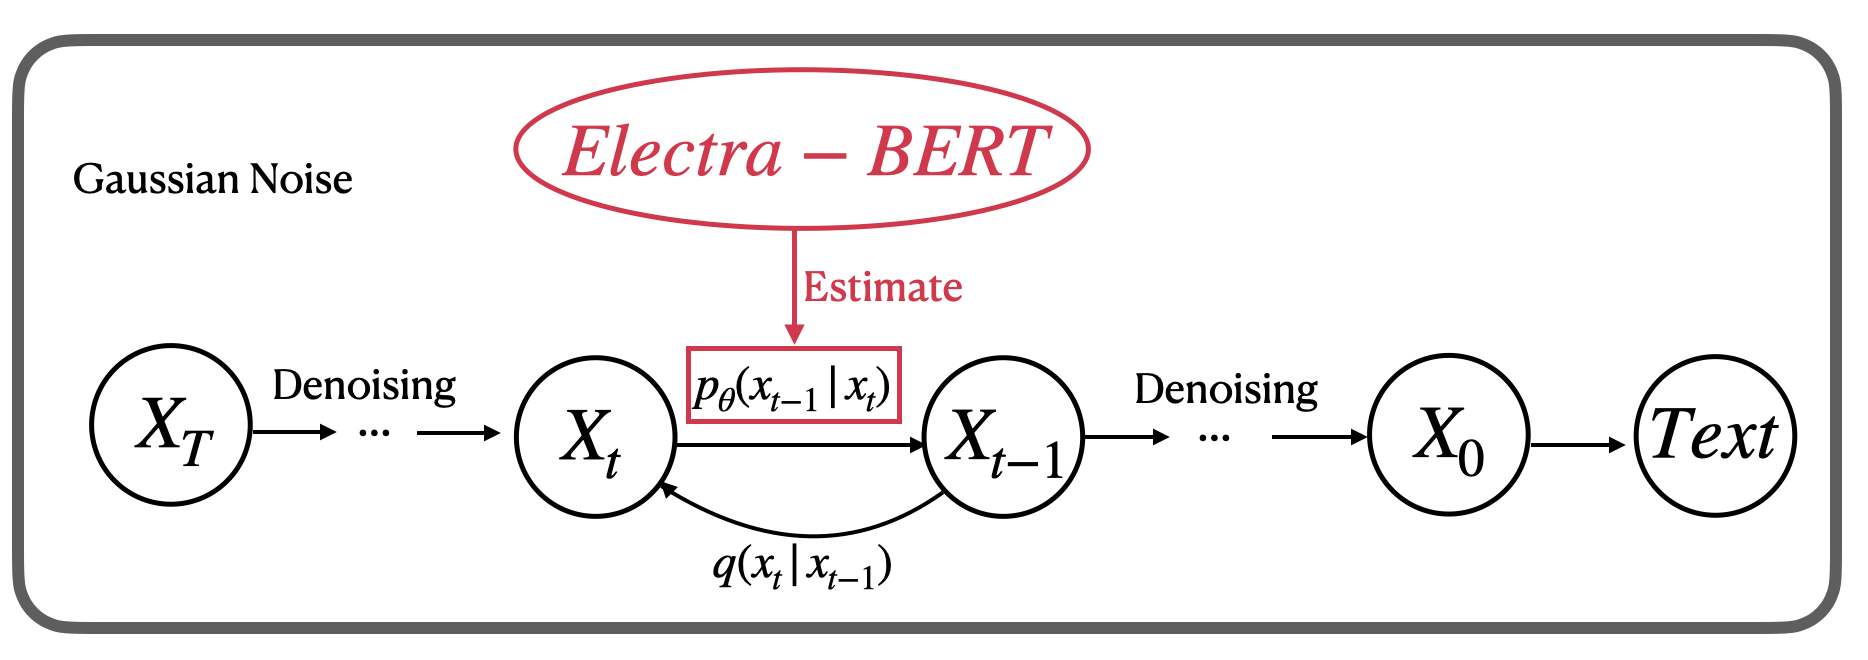
\includegraphics[width=12cm]{Electra.png}
     \caption{Graphical representation of the diffusion model with Electra-BERT.}\label{Fig:Data1}
   \end{minipage}\hfill
\end{figure}

In the diffusion model, to estimate $p_{\theta}(x_{t-1}|x_t)$, we can use any neural networks in theory since sophisticated or complicated neural networks can approximate any real-value functions. Given the nature that text is a sequence, we choose to use the sequential model for the task. In this paper, we trained the Diffusion-LM model using Transformers, such as Bidirectional Encoder Representations from Transformers (BERT) in [9] and Electra-BERT in [10].


\section{Results}

We shall now discuss the outcomes of our project experiments.

\subsection{Experiments setting}

Our project's best result was obtained by training under the following background and set of parameters. We trained the model with 1,000 iterations and employed forward/reverse steps of 20,000. The learning rate was 0.0001, and the transformer fed into each reverse step was BERT and Electra-BERT. 

We discovered that the pattern of overfitting on generated output occurred at around 800 and 1500 iterations for the model with BERT and the model with Electra-BERT respectively. We also discovered that the results from the model trained with BERT were more coherent than the model trained with Electra-BERT. Therefore, in this paper, we showcase and discuss the audio generated by the model using BERT under 800 iterations. 


\subsection{Evaluation Metrics}


We employ bit-per-word (bpw) [11] as the evaluation metric to quantitatively evaluate the quality of generated text file. It is similar to the cross entropy and shown below:

\begin{equation}
    \begin{split}
        bpw(token) = \frac{1}{T}\sum\limits_{t=1}^{T}H(P_t, \hat{P}_t) 
        & = - \frac{1}{T} \sum\limits_{t=1}^{T}
        \sum\limits_{c=1}^{n} P_t(c)\log_2\hat{P_t}(c)\\
        & = - \frac{1}{T} \sum\limits_{t=1}^{T}\log_2\hat{P}_t(x_t)
    \end{split}
\end{equation}

bpw is beneficial for us to evaluate the quality of the generated sentences under the assumption that if a sentence is full of less-frequent words then it is uncommon to generate this sentence. In this way, it is more economical to compress the frequent words using less bits and compress the less-frequent words using more bits. Hence, there's a negative relationship between the compression size and the probability (frequency) of the generated sentences.

We summarize and compare the result of Diffusion-LM using BERT and Electra below:\\

\begin{tabular}{ |p{5cm}||p{2cm}||p{3cm}||p{3cm}|}
 \hline
 \multicolumn{4}{|c|}{Results} \\
 \hline
 Model & Iterations & Steps & bits-per-word\\
 \hline
  Diffusion-LM using BERT  & 800  & 2000 &  0.00003   \\
 Diffusion-LM using BERT  & 1000  & 2000 &  0.00004   \\
 Diffusion-LM using BERT  & 2000 &  2000 & 0.00007  \\
 Diffusion-LM using Electra & 1000 &  2000 & 0.00020  \\
 Diffusion-LM using Electra & 2000 &  2000 & 0.00030  \\
 \hline
\end{tabular}\\

The lower bpw means the compression size of the sentence is small, which means the sentence is more frequent based on the negative relationship mentioned above. The result is not surprising since Electra has much less parameters than BERT and sacrifice part of its accuracy. The reason we want to try Electra is we aim to make the Diffusion-LM more practical without training for a long time, and make it trainable even in the single consumer CPU or GPU. 

\subsection{MIDI Visualization}

The following figure shows the MIDI file generated by our trained model. 


\begin{figure}[!htb]
   \begin{minipage}{1\textwidth}
     \centering
     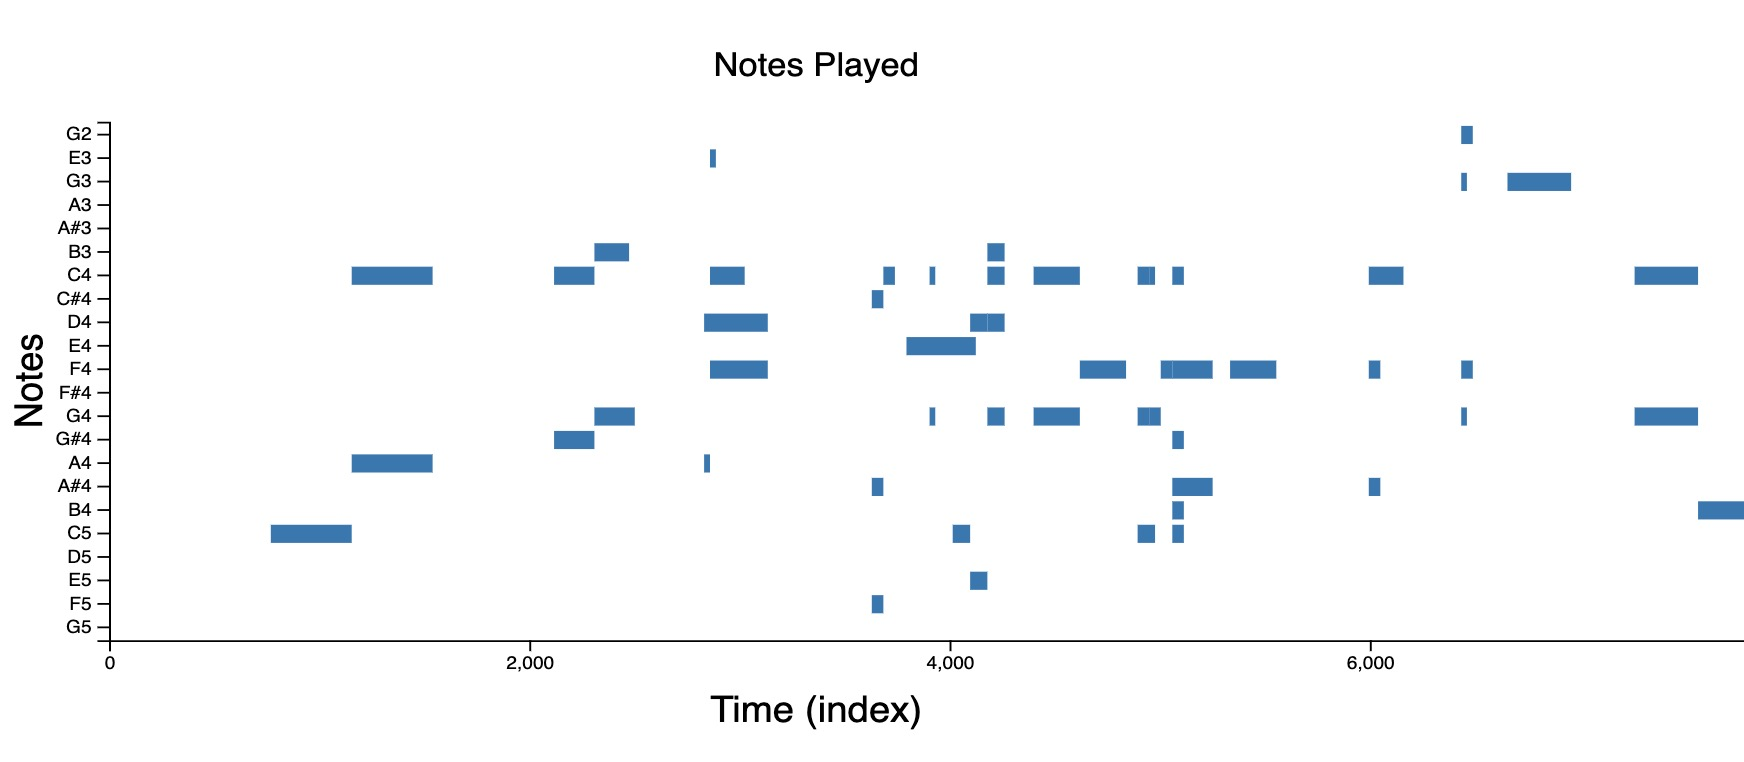
\includegraphics[width=9cm]{note.jpeg}
     \caption{Sample Generated MIDI output with 800 checkpoints}\label{Fig:Data1}
   \end{minipage}\hfill
\end{figure}


\subsection{Waveform Visualization}

The following diagram, figure 5 below, presents a more straightforward representation of the music generated by the model. From the waveform below, there is some gaps between each note, which results in the incoherence of our music.  

\begin{figure}[!htb]
   \begin{minipage}{1\textwidth}
     \centering
     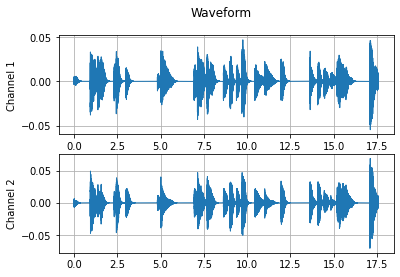
\includegraphics[width=9cm]{9-midi-waveform.png}
     \caption{Waveform visualization of the generated MIDI file}\label{Fig:Data1}
   \end{minipage}\hfill
\end{figure}


\section{Conclusion}

In conclusion, we can say that we were successful in our methodology to generate discrete music by optimizing a language model. However, we can further improve the quality of our generated music. One big drawback of our current model is that we are training on a relatively small-sized dataset. Use of a larger dataset and a better data augmentation technique will boost the performance of our model. One thing to also note is that we froze the controllable classifier that formulated a big part in the architecture of the Diffusion-LM model. For future experiments, we propose to unfreeze this functionality to improve the quality of generation by the model.. \\


\section*{References}
{
\small
[1] Zala ́n Borsos, Raphae ̈l Marinier, Damien Vincent, Eugene Kharitonov, Olivier Pietquin, Matt Shar- ifi, Olivier Teboul, David Grangier, Marco Tagliasacchi \& Neil Zeghidour. Audiolm: a language modeling approach to audio generation. arXiv preprint arXiv:2209.03143, 2022. 

[2] A. van den Oord, S. Dieleman, H. Zen, K. Simonyan,
O. Vinyals, A. Graves, N. Kalchbrenner, A. W. Senior,
and K. Kavukcuoglu, “WaveNet: A generative model
for raw audio,” in The 9th ISCA Speech Synthesis Workshop, Sep. 2016, p. 125.

[3] A. van den Oord, S. Dieleman, H. Zen, K. Simonyan,
O. Vinyals, A. Graves, N. Kalchbrenner, A. W. Senior,
and K. Kavukcuoglu, “WaveNet: A generative model
for raw audio,” in The 9th ISCA Speech Synthesis Workshop, Sep. 2016, p. 125.

[4] C. Donahue, J. J. McAuley, and M. S. Puckette, “Adversarial audio synthesis,” in 7th International Conference on Learning Representations (ICLR), May 2019.

[5] P. Dhariwal, H. Jun, C. Payne, J. W. Kim, A. Radford,
and I. Sutskever, “Jukebox: A generative model for
music,” arXiv preprint arXiv:2005.00341, 2020.

[6] J. H. Engel, K. K. Agrawal, S. Chen, I. Gulrajani,
C. Donahue, and A. Roberts, “GANSynth: Adversarial neural audio synthesis,” in 7th International Conference on Learning Representations (ICLR), May 2019.

[7] Xiang Lisa Li, John Thickstun, Ishaan Gulrajani, Percy Liang, and Tatsunori B Hashimoto. 2022. Diffusion-LM Improves Controllable Text Generation. arXiv preprint arXiv:2205.14217, 2022.

[8] Jonathan Ho, Ajay Jain, and Pieter Abbeel. Denoising diffusion probabilistic models. In Advances in Neural Information Processing Systems, pages 6840–6851, 2020.

[9] Jacob Devlin, Ming-Wei Chang, Kenton Lee, and Kristina Toutanova. 2018. BERT: Pre-training of deep bidirectional transformers for language understanding. arXiv:1810.04805. Retrieved from https://arxiv.org/abs/1810.04805.

[10] Kevin Clark, Minh-Thang Luong, Quoc V. Le, and Christopher D Manning. 2020. Electra: Pre-training text encoders as discriminators rather than generators. Retrieved from https://arXiv:2003.10555.

[11] Alex Graves. Generating sequences with recurrent neural networks. ArXiv Preprint arXiv:1308.0850, 2013.

[12] Jeff Ens, Philippe Pasquier. "MMM : Exploring Conditional Multi-Track Music Generation with the Transformer". 	arXiv:2008.06048

[13] Aaron Van den Oord, Nal Kalchbrenner, Lasse Espeholt, Oriol Vinyals, Alex Graves, et al. 2016. Conditional image generation with pixelcnn decoders. In NeurIPS.

[14] Zalan Borsos, Rapha ´ el Marinier, Damien Vincent, Eugene Kharitonov, Olivier Pietquin, Matt Shar- ¨
ifi, Olivier Teboul, David Grangier, Marco Tagliasacchi, and Neil Zeghidour. Audiolm: a language modeling approach to audio generation. arXiv preprint arXiv:2209.03143, 2022.

[15] Gautam Mittal, Jesse Engel, Curtis Hawthorne, and Ian Simon. Symbolic music generation
with diffusion models. arXiv preprint arXiv:2103.16091, March 2021.

[16] M. Pasini and J. Schluter, “Musika! fast infinite waveform music generation,” CoRR, vol. abs/2208.08706, 2022. [Online]. Available:
https://doi.org/10.48550/arXiv.2208.08706



}




\end{document}
